
\documentclass[11pt]{exam} % https://www.ctan.org/pkg/exam?lang=en

\usepackage[lmargin=1.in,rmargin=1.in,tmargin=1.in,bmargin=1in]{geometry}
\usepackage{setspace}
\usepackage[pdftex]{graphicx}
\usepackage{titling}
\usepackage[
	pdfauthor={Brian Weinstein},
	pdftitle={Homework 4},
	bookmarks=true,
	colorlinks=true,
	linkcolor=blue,
	urlcolor=blue,
	citecolor=blue,
	pdftex,
	linktocpage=true
	]{hyperref}
\usepackage[textsize=tiny]{todonotes}
\usepackage{float}
\setlength\parindent{0pt}
\usepackage{lipsum}
\usepackage{amsmath}


\qformat{\textbf{Problem \thequestion: \thequestiontitle}\quad \hfill}


\pagestyle{headandfoot}
\runningheadrule
\firstpageheader{}{}{}
\runningheader{\theauthor}{\thetitle}{\thedate}
\firstpagefooter{}{\thepage}{}
\runningfooter{}{\thepage}{}


\usepackage{xcolor}
\usepackage{adjustbox}
\usepackage{verbatim}
\definecolor{shadecolor}{rgb}{.9, .9, .9}

\newenvironment{code}%
   {\par\noindent\adjustbox{margin=1ex,bgcolor=shadecolor,margin=0ex \medskipamount}\bgroup\minipage\linewidth\verbatim}%
   {\endverbatim\endminipage\egroup}

\newenvironment{codeSmall}%
   {\par\noindent\adjustbox{margin=1ex,bgcolor=shadecolor,margin=0ex \medskipamount}\bgroup\minipage\linewidth\verbatim\footnotesize}%
   {\endverbatim\endminipage\egroup}

\newcommand{\ramsey}{\href{http://www.statisticalsleuth.com/}{Ramsey }}



\begin{document}


\title{STAT W4201 001, Homework 4}
\author{Brian Weinstein (bmw2148)}
\date{Feb 24, 2016}
\maketitle

Code is attached here and also posted at \href{https://github.com/BrianWeinstein/advanced-data-analysis}{https://github.com/BrianWeinstein/advanced-data-analysis}. Where relevant, code snippets and output are are included in-line.

\begin{questions}



\titledquestion{\ramsey 5.23}

The data provides overwhelming evidence that the mean oxygen isotopic composition in the 12 bone samples are different (a p-value of $9.7\times 10^{-7}$ from a one-way analysis of variance (ANOVA) F-test).

The ANOVA table testing for a difference in mean oxygen isotopic composition is shown below, and a boxplot of oxygen composition for each bone is shown in Figure \ref{fig:1}.

\begin{center}
  \begin{tabular}{ l c c c c c}
    Source of Variation & Sum of Squares & d.f. & Mean Square & F-Statistic & p-Value \\ \hline \hline
    Between Groups & 6.0675 & 11 & 0.55159 & 7.4268 & $9.73\times 10^{-7}$ \\
    Within Groups & 2.9708 & 40 & 0.07427 & & \\ \hline
    Total & 9.0383 & 51 & & &
  \end{tabular}
\end{center}

\begin{figure}[!h]
	\centering
	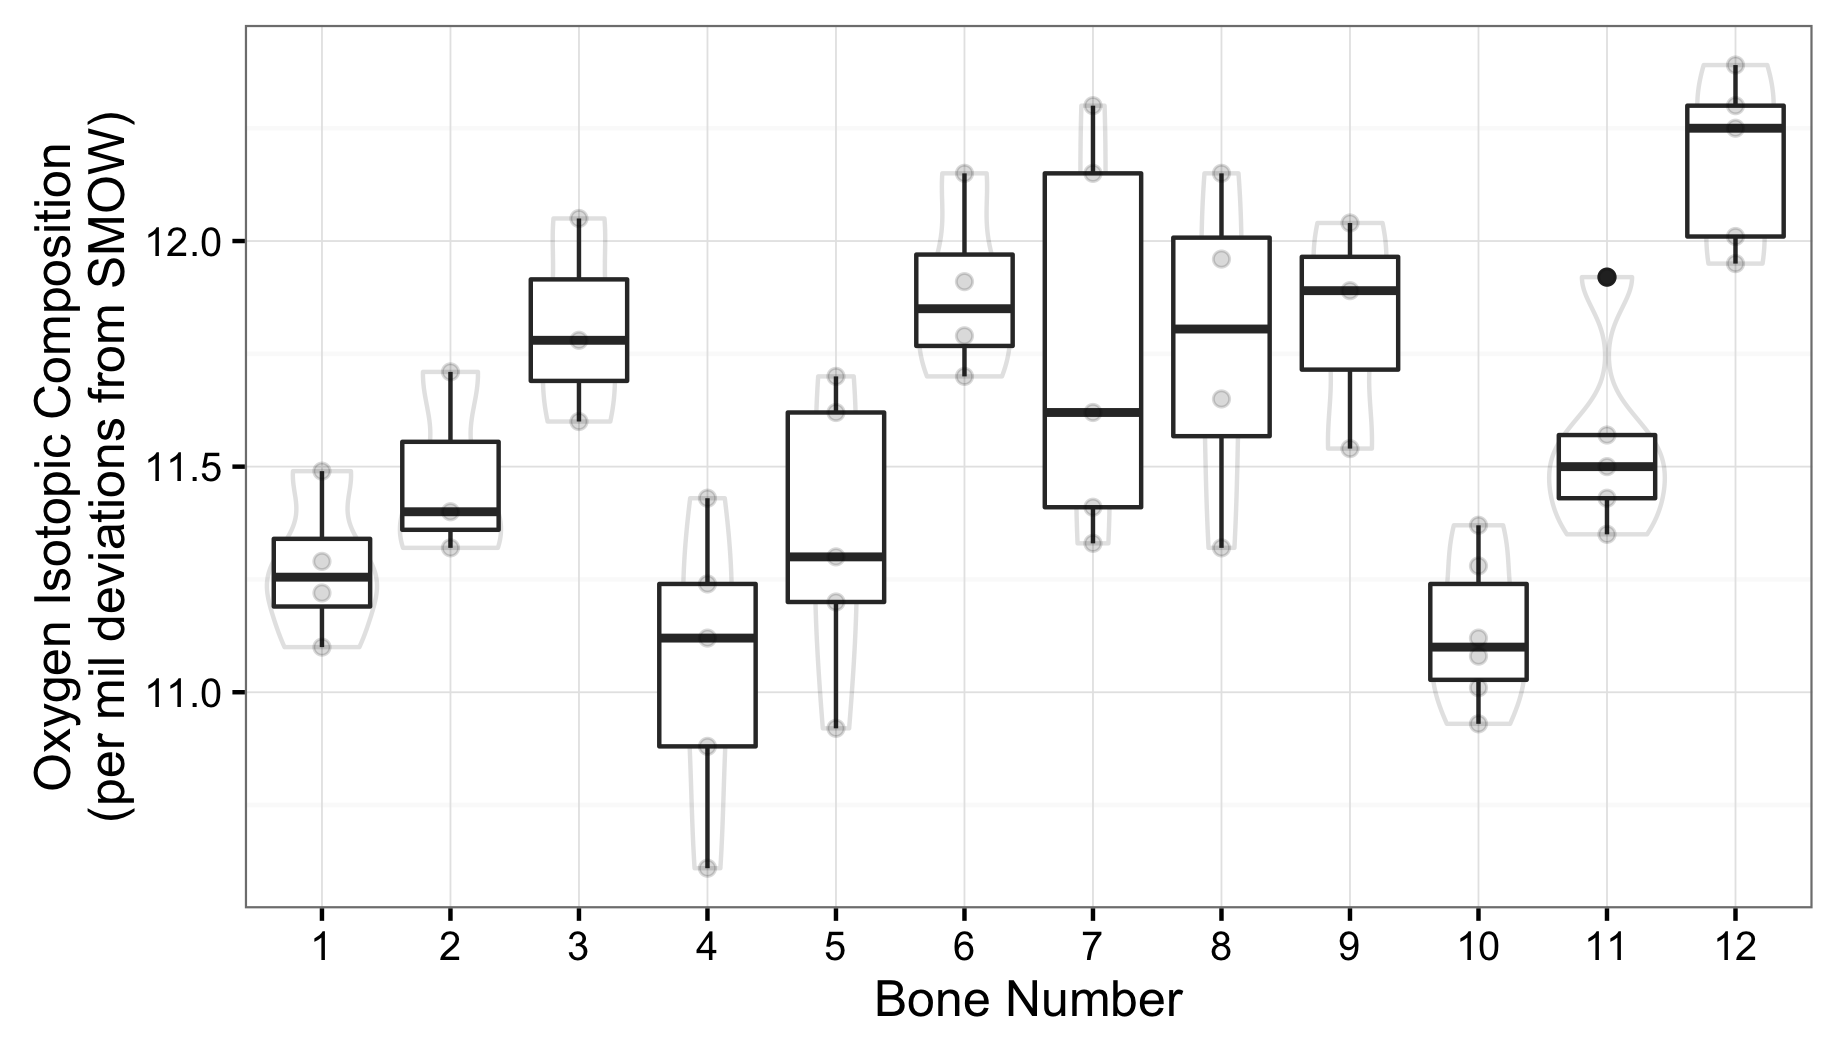
\includegraphics[width=4.25in]{1.png}
	\caption{Oxygen Isotopic Composition (per mil deviations from SMOW) for twelve bones of a single Tyrannosaurus rex specimen.}
	\label{fig:1}
\end{figure}



\titledquestion{\ramsey 5.25}



\titledquestion{\ramsey 6.12}



\titledquestion{\ramsey 6.15}



\titledquestion{\ramsey 6.16}



\titledquestion{\ramsey 6.23}




\end{questions}

\listoftodos

\end{document}